\documentclass{report}

\usepackage{booktabs}
\usepackage{float}
\usepackage{comment}
\usepackage{graphicx} 
\usepackage{amsthm} 
\usepackage{amsfonts}
\usepackage{pdfpages} 
\usepackage{siunitx} 
\usepackage{mhchem}
\usepackage{subfloat}
\usepackage{fullpage}
\usepackage{array}
\usepackage[toc,page]{appendix}

\newcommand{\ecoli}{\textit{E. coli}}
\newcommand{\ecloni}{\textit{E. cloni 10g}} 
\newcommand{\bsub}{\textit{B. subtilis}} 
\newcommand{\pbad}{P$_{BAD}$} 
\newcommand{\plux}{P$_{LUX}$}
\newcommand{\etal}{\textit{et al.}} 
\newcommand{\invivo}{\textit{in vivo}}
\newcommand{\invitro}{\textit{in vitro}} 
\newcommand{\csix}{3OC6HSL}

\newcommand{\tred}[1]{\textcolor{red}{#1}}
\newcommand{\tgr}[1]{\textcolor{green}{#1}}

% Units
\DeclareSIUnit{\molar}{M} 
\newcommand{\ul}{\si{\micro\litre}} 
\newcommand{\um}{\si{\micro\metre}}
\newcommand{\ml}{\si{\milli\litre}} 
\newcommand{\nm}{\si{\nano\metre}} 
\newcommand{\ugml}{\si{\micro\gram\per\milli\litre}} 
\newcommand{\degC}{\si{\degreeCelsius}}

% Misc
\newcommand{\tenx}{\ensuremath{10\times}}
\newcommand{\fortyx}{\ensuremath{40\times}}
\newcommand{\sixtyx}{\ensuremath{60\times}}
\newcommand{\hundredx}{\ensuremath{100\times}}
\newcommand{\odsix}{\ensuremath{\textrm{OD}_{600}}}
\newcommand{\Pspo}{\ensuremath{\textrm{P}_{\textrm{\scriptsize SPO1-26}}}}

% Matrix/ vector shit
\let\oldhat\hat 
\renewcommand{\vec}[1]{\mathbf{#1}}
\renewcommand{\hat}[1]{\oldhat{\mathbf{#1}}}
\let\oldcaption\caption
%\renewcommand{\caption}[2][]{\oldcaption[#1]{\small\textbf{#1.} #2\normalsize}}
\renewcommand{\caption}[2][]{\oldcaption[#1]{\textbf{#1.} #2}}

\newcommand{\mat}{\mathbf} 
\newcommand{\invmat}[1]{\mat{#1}^{-1}}
\newcommand{\deltap}{\Delta \vec{p}} 
\newcommand{\deltaL}{\Delta \vec{L}}
\newcommand{\deltag}{\Delta g} 
\newcommand{\Iinv}{\mat{I}^{-1}}
\newcommand{\Minv}{\mat{M}^{-1}}
\newcommand{\crossmat}[1]{{\left[#1\right]}_{\times}}

\newtheorem{remark}{Remark} 
\newtheorem*{note}{Note} 

\begin{document} 

\chapter{Biophysical modelling of rod-shaped bacterial cells}
\section{Biophysical model}
The measurements of individual cells in microcolonies of \ecoli\
presented above are consistent with the overview presented by
Koch~\cite{Koch:1995} that cells have fixed diameter and grow only along their
major axis, and the findings of Wang \etal~\cite{Wang:2010} showing that cells
are equally bisected on division.  The observation that cell diameter is
constant suggests that cells are \textit{rigid} except in the direction of
their growth axis. Following this suggestion, we formulated a simple model of
cellular growth on an agar substrate as follows: 
\begin{enumerate} 
\item Cells are rigid elongating capsules~\cite{Koch:1995}.  
\item Viscous drag dominates inertia; cells are non-motile and move only when
subjected to a force~\cite{Purcell:1977}.  
\item The distribution of cell lengths at division is constant, and each cell
divides in half~\cite{Wang:2010,Koch:1995}.    
\item Each cell's unconstrained growth rate is proportional to its
length~\cite{Wang:2010}.  
\item Growth is constrained by forces between cells and from viscous drag from
the substrate (figure \ref{fig:model}).  The ratio of the work required to
constrain growth to the work required to move a cell is defined by a parameter
$\Gamma$.  
\end{enumerate}
In a rigid body mechanics model objects cannot be deformed and are completely
represented by their position and orientation. We extend this formulation by
allowing cell length to vary, adding an extra degree of freedom to accommodate
growth.

\section{Mathematical description of biophysical model}
\subsection{Motion of cells due to applied impulse} 
Bacterial cells are modelled as capsule-shaped rigid bodies, that is cylinders
capped with hemispherical ends. Each cell is represented by its
position, orientation and length ($\vec{x}$, $\vec{\theta}$, $l$), and the
associated linear, angular, and growth velocity ($\vec{v}_\textrm{lin}$,
$\vec{w}$, $v_\textrm{growth}$). Here $v_\textrm{growth}$ is the
linear growth rate $dl/dt$. By extension of the usual rigid-body
formulation, we define the generalised position of a cell as
$\tilde{\vec{x}} = 
\left(\begin{array}{lll}\vec{x} & \vec{\theta} & l \end{array}\right)^T$, and
the generalised velocity as $\tilde{\vec{v}} = d\tilde{\vec{x}}/dt =  
\left(\begin{array}{lll}\vec{v}_\textrm{lin} & \vec{w} & v_\textrm{growth} \end{array}\right)^T$.
Similarly there is a generalised momentum associated with the motion of the cell 
$\tilde{\vec{p}} =  
\left(\begin{array}{lll}\vec{p} & \vec{L} & g \end{array}\right)^T$, with
linear, angular and growth components.
Cells grow by
acquiring growth momentum $g$ which causes extension in length.  For a physically
possible arrangement of cells, this extension in length cannot cause the cells
to overlap or intersect, leading to a system of constraints. It is the solution
of this system of constraints, which is derived below, that results in
computation of the correct arrangement of cells during colony growth.

In appendix \ref{app:eqmot} I show with the assumptions listed above, under a generalised impulse $\Delta
\tilde{\vec{p}}_i$ the change in generalised position of a cell $\Delta
\tilde{\vec{x}}_i$ is
determined by a matrix $\mat{M}_i$ such that:
\begin{align}
\Delta \tilde{\vec{ x}}_i &=
\invmat{M_i} \Delta \tilde{\vec{p}}_i \\
&=
\left[
\begin{array}{ccc}
\textrm{diag}(\frac{1}{\mu l_0}) & 0 & 0 \\
0 & \frac{12\mat{P_i}}{\mu l_0^3} & 0 \\
0 & 0 & \frac{1}{\gamma} \\
\end{array}
\right]
\left[
\begin{array}{l}
\deltap_i \\ \deltaL_i \\ \deltag_i
\end{array}
\right]%\\
%&=
%\mat{M}^{-1}\deltap
\label{eqn:motion2}
\end{align}
where $l_0$ is the length of cell $i$, and $\invmat{M_i}$ is written in block form - $\textrm{diag}(\frac{1}{\mu l_0})$
and $\frac{12\mat{P}}{\mu l_0^3}$ are $(3\times3)$, and $\frac{1}{\gamma}$ is
$(1\times1)$. The matrix $\mat{P}$ is the projection onto
the plane perpendicular to the cell axis $\hat{\vec{a}}$, i.e. $\mat{P}\deltaL
\equiv \deltaL -
\hat{\vec{a}}(\hat{\vec{a}} \cdot \deltaL)$.

\begin{note}
There are 7 degrees of freedom for each cell, hence generalised position,
velocity and impulse are $7\times1$ vectors. There are 3 components of centroid
position/velocity/impulse ($\vec{x}$, $\vec{v}_\mathrm{lin}$, $\Delta \vec{p}$),
3 components of angular position/velocity/impulse ($\vec{\theta}$, $\vec{w}$,
$\deltaL$), and 1 component of length/growth rate/growth impulse ($l$,
$v_\textrm{growth}$, $g$).
\end{note}

\begin{center}
\begin{figure}[p]\centering
\subfloat[]{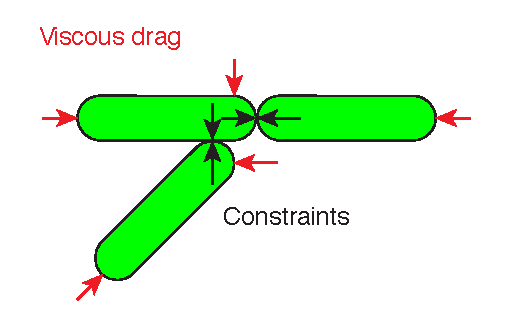
\includegraphics[scale=0.75]{cellforces}}\qquad
\subfloat[]{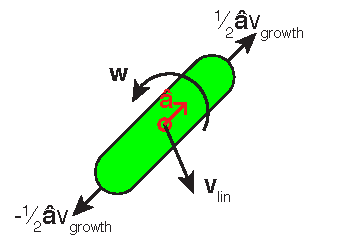
\includegraphics{cellvel}}
\caption[Biophysical model of rod-shaped bacteria, forces and motion]
{Biophysical model of rod-shaped bacteria considers each cell as a capsule
(shown in two-dimensions). Forces on each cell (a) are generated by viscous drag
(red) and constraints at cell-cell contacts (black). The velocity of a point on
a cell consists of multiple components (b): the cell centre of mass (red circle)
moves with linear velocity $\vec{v}_\textrm{lin}$, the cell rotates with angular
velocity $\vec{w}$, and grows at instantaneous linear rate $v_\textrm{growth}$ causing all points to
move away from the centre of mass along the axis ($\hat{\vec{a}}$).}
\label{fig:model}
\end{figure}
\end{center}

\begin{center}
\begin{figure}[p]\centering
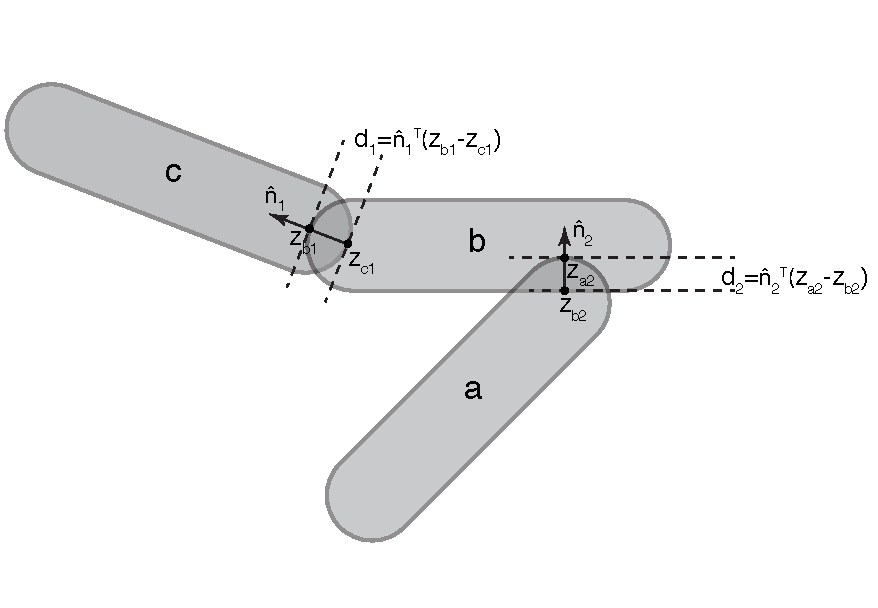
\includegraphics[scale=0.75]{celloverlap}
\caption{}
\label{fig:overlap}
\end{figure}
\end{center}

\subsection{Motion of points on cell surfaces}
We described above the change in generalised position of a cell due to a
generalised impulse, that is the change in its centroid location, angular
orientation, and length. Now consider the motion of a point on the
surface of this cell due to the change in generalised position. This point is
positioned according to vector $\vec{q}$ from the center
of the capsule $\vec{x}_i$, which has axis $\hat{\vec{a}}_i$.  Its original position is
$\vec{q}_w = \vec{x}_i + \vec{q}$.
For small displacments the cell axis $\hat{\vec{a}}_i$, the associated
projection matrix $\mat{P}_i$, and the cell length $l_0$ remain approximately constant, and
\[
\Delta \vec{q}_w \approx
\Delta \vec{ x_i} +
(\Delta \vec{\theta_i}\times\vec{q}) +
\frac{\Delta l_i}{l_0} \left(\hat{a}_i\cdot\vec{q}\right)\hat{a}_i
\]

And substituting from equation \ref{eqn:motion}:
\begin{align*}
\Delta \vec{ q}_w &\approx
\Delta \vec{ x_i} -
(\vec{q} \times \Delta \vec{\theta_i}) +
\frac{\left(\hat{a}_i\cdot\vec{q}\right)\hat{a}_i}{l_0} \Delta l_i \\
&\approx
\frac{1}{\mu l_0} \deltap_i -
(\vec{q} \times \frac{12\mat{P}_i}{\mu l_0^3}\deltaL_i) +
\frac{\left(\hat{a}_i\cdot\vec{q}\right)\hat{a}_i}{l_0}\frac{\deltag_i}{\gamma}
\end{align*}

Now project this vector along the direction vector $\hat{n}$ of interest to get
the position change in a particular direction:
\begin{align*}
\Delta q_{\hat{n}}
&=
\hat{n} \cdot
\left(
\frac{1}{\mu l_0} \deltap_i -
(\vec{q} \times \frac{12\mat{P}_i}{\mu l_0^3}\deltaL_i) +
\frac{\left(\hat{a}_i\cdot\vec{q}\right)\hat{a}_i}{l_0}\frac{\deltag_i}{\gamma}
\right) \\
&=
\frac{1}{\mu l_0}\hat{n}\cdot\deltap_i -
\frac{12}{\mu l_0^3}\left(\hat{n}\times\vec{q}\right)\cdot \mat{P}_i\deltaL_i +
\frac{\left(\hat{n}\cdot\hat{a}_i\right)\left(\hat{q}\cdot\hat{a}_i\right)}{l_0}\frac{\deltag_i}{\gamma} \\
\end{align*}

Which can be written in block matrix form as:
\begin{align*}
\Delta  q_{\hat{n}}
&=
\left[
\begin{array}{lll}
\hat{n}^{\textrm{T}} & -\left(\hat{n}\times\vec{q}\right)^{\textrm{T}} &
\frac{\left(\hat{n}\cdot\hat{a}_i\right)\left(\vec{q}\cdot\hat{a}_i\right)}{l_0} \\
\end{array}
\right]
\left[
\begin{array}{lll}
\frac{1}{\mu l_0} & 0 & 0 \\
0 & \frac{12\mat{P}_i}{\mu l_0^3} & 0 \\
0 & 0 & \frac{1}{\gamma} \\
\end{array}
\right]
\left[
\begin{array}{l}
\deltap_i \\ \deltaL_i \\ \deltag_i
\end{array}
\right]\\
&= \mat{B}_{\hat{n},\vec{q},i}\invmat{M}_i\Delta\tilde{\vec{p}}_i
\end{align*}

Here $\mat{B}_{\hat{n},\vec{q},i}$ is a matrix which represents 
the geometric effect of a generalised position change on a point at $\vec{q}$
from the centre of cell $i$ along direction $\hat{n}$, and
matrix $\invmat{M}_i$ is the inverse drag matrix for cell $i$. 
The expression for $\Delta q_{\hat{n}}$ represents the motion of the surface point
at position $\vec{q}$ relative to the capsule centre in the direction $\hat{n}$ that
results from application of generalised impulse $\Delta \tilde{\vec{p}}$. This quantity is central
to the formation of the constraints explained below.

\subsection{Effect of a set of applied impulses on cell-cell overlap distances}
Now consider two overlapping capsules $a$ and $b$, forming contact $k$. We find the contact points on
each cell $\vec{z}_{ak}$ and $\vec{z}_{bk}$ as described above (figure \ref{fig:overlap}). The
change in overlap distance $d_k$ is the difference in the movement of these
contact points along the contact normal $\hat{n}_k$. That is for generalised
impulses $\Delta\tilde{\vec{p}}_a$ and $\Delta\tilde{\vec{p}}_b$ applied to cell
$a$ and $b$,
\begin{align*}
\mat{B}_{ak} \Minv_a \Delta\tilde{\vec{p}}_a -
\mat{B}_{bk} \Minv_b \Delta\tilde{\vec{p}}_b
&=
\Delta d_k \\
\end{align*}
where $\mat{B}_{ak}$
and $\mat{B}_{bk}$ are as $\mat{B}$ matrices as defined above using the contact normal 
$\hat{\vec{n}}_k$ as the direction vector, and the relative positions of
$\vec{z}_{ak}$ and $\vec{z}_{bk}$ from their respective cells.  Viewed in block matrix form:
\begin{align*}
\left[
\begin{array}{ll}
\mat{B}_{ak} \Minv_a &
-\mat{B}_{bk} \Minv_b \\
\end{array}
\right]
\left[
\begin{array}{l}
\Delta\tilde{\vec{p}}_a \\
\Delta\tilde{\vec{p}}_b \\
\end{array}
\right]
=
\left[
\begin{array}{l}
\Delta d_k
\end{array}
\right]
\end{align*}

In a system of multiple cells, there will be one such equation for each contact $k$ between two capsules.
To solve all these equations simultaneously, each equation becomes a
row in a matrix equation.  For example, with four cells and
three contacts, the
system might be:
\begin{align*}
\left[
\begin{array}{llll}
\mat{B}_{a1}\Minv_1 & -\mat{B}_{b1}\Minv_2 & 0 & 0 \\
\mat{B}_{a2}\Minv_1 & 0 & -\mat{B}_{c2}\Minv_3 & 0 \\
0 & \mat{B}_{b3}\Minv_1 & 0 & -\mat{B}_{d3}\Minv_4 \\
\end{array}
\right]
\left[
\begin{array}{c}
\Delta\tilde{\vec{p}}_a\\
\Delta\tilde{\vec{p}}_b\\
\Delta\tilde{\vec{p}}_c\\
\Delta\tilde{\vec{p}}_d\\
\end{array}
\right]
=
\left[
\begin{array}{c}
\Delta d_1\\
\Delta d_2\\
\Delta d_3\\
\end{array}
\right]
\end{align*}

\begin{align*}
\left[
\begin{array}{llll}
\mat{B}_{a1} & -\mat{B}_{b1} & 0 & 0 \\
\mat{B}_{a2} & 0 & -\mat{B}_{c2} & 0 \\
0 & \mat{B}_{b3} & 0 & -\mat{B}_{d3} \\
\end{array}
\right]
\left[
\begin{array}{llll}
\Minv_1 & 0 & 0 & 0 \\
0 & \Minv_2 & 0 & 0 \\
0 & 0 & \Minv_3 & 0 \\
0 & 0 & 0 & \Minv_1  \\
\end{array}
\right]
\left[
\begin{array}{c}
\Delta\tilde{\vec{p}}_a\\
\Delta\tilde{\vec{p}}_b\\
\Delta\tilde{\vec{p}}_c\\
\Delta\tilde{\vec{p}}_d\\
\end{array}
\right]
=
\left[
\begin{array}{c}
\Delta d_1\\
\Delta d_2\\
\Delta d_3\\
\end{array}
\right]\\
\end{align*}

and writing the system with single collected matrices and vectors,

\begin{equation*}
\mat{B} \invmat{M} \Delta \tilde{\vec{p}} = \Delta \vec{d}
\end{equation*}

\begin{note}
The elements $\mat{B}_{ij}\invmat{M}_i$ are computed by the \texttt{to\_ents}
(positive) and
\texttt{fr\_ents} (negative) arrays ($7\times1$ vectors stored in
\texttt{float8}) which are stored for each cell for each contact it
is involved in. We consider contacts to be directed from low to high index, and
so only the cell with the lowest index in each contact stores and calculates
these entries.
\end{note}

\begin{note}
In the analysis above I have split the matrices $\mat{B}$ and $\invmat{M}$, but
currently the combination $\mat{B}\invmat{M}$ is computed. It may be better to
split it so that we can more easily compute other forms of $\mat{B}$, e.g. for adhesion (see
below). Application of $\invmat{M}$ is already implemented by
\texttt{compute\_Minvx}.
\end{note}


\subsection{Growth of cells generates impulses to prevent overlap}
Growth of cells during a discrete time-step $\Delta t$ is modelled by simply
increasing the length of each cell by $v_\textrm{growth}\Delta t$. This
causes cells to overlap (figure \ref{fig:overlap}). For a physically correct
arrangement of cells, reaction or constraint forces must be generated to
eliminate this overlap.

A capsule of total length $l$ and radius $r$
is defined as the locus of points within a
radius $r$ of the line segment of length $l-2r$ along its axis.
When two such capsules overlap, we define the points of intersection on each cell
($\vec{z}$ in figure \ref{fig:overlap}) as follows. First we find the closest points
on each cell's axis line segment. The line joining these points then intersects
each cell surface at points labelled $\vec{z}$, where it is normal to the surface.
Hence we have defined contact points on each cell, and the normal to the contact
$\hat{\vec{n}}$. The distance of overlap $d$ for each contact is then determined
by the distance between the contact points along the contact normal direction
(figure \ref{fig:overlap}). 

In order to constrain the system of cells to produce
a physically possible, non-overlapping arrangement, we must find the 
impulse applied to each cell $\Delta \tilde{\vec{p}}$ that produces a change in
the overlap distance so that $d=0$ for each contact. 
We have just described how these overlap distances are changed by a set of
applied impulses, and so we can now formulate the constraint system.

\subsection{Constraint formulation}
To form a physically possible arrangement of cells after increasing their length
we wish to apply constraint impulses to cells such that
\begin{eqnarray*}
\vec{d} + \Delta \vec{d} &=& 0\\
\Delta \vec{d} &=& -\vec{d}
\end{eqnarray*}
As shown above the change in overlaps $\Delta \vec{d}$ produced by a set of
generalised impulses $\Delta \tilde{\vec{p}}$ means that
\[
\mat{B}\invmat{M}\Delta\tilde{\vec{p}} = \mat{A}\Delta\tilde{\vec{p}} = \Delta
\vec{d}
\]
where $\mat{A}$ is a block matrix $n_{\textrm{contacts}} \times
n_{\textrm{cells}}$, $\Delta\tilde{\vec{p}}$ is a block vector $n_{\textrm{cells}} \times 1$ and
$\vec{d}$ is  $n_{\textrm{contacts}}\times 1$. Hence the constrained system is
given by:
\[
\mat{A}\Delta\tilde{\vec{p}} + \vec{d} = 0
\]
Hence we have formulated the system of constraints as a linear system. Given the
solution of this system, the change in generalised position of each cell is then $\Minv \Delta\tilde{\vec{p}}$.
However it is clear that in general this linear system does not have a unique solution.
To see this consider that cells may move perpendicular to the normal(s) of their
contact(s) without affecting $\Delta \vec{d}$.

\subsection{Energy minimising solution}
The least squares solution of the constraint system is:
\[\underset{\deltap}{\operatorname{argmin}}
\left\{
\left\|\mat{A}\Delta\tilde{\vec{p}} + \vec{d}\right\|^2 \right\} \]
%\[\mat{A}^{\textrm{T}}\mat{A}\deltap = -\mat{A}^{\textrm{T}}\vec{d}\]
where the expression $\mat{A}\Delta\tilde{\vec{p}} + \vec{d}$ is the vector of overlap
distances of each contact after application of impulses $\Delta \tilde{\vec{p}}$. If we interpret the least-squares
solution as an energy minimising solution, where the energy is
associated with the overlap of each contact. If the overlap at each
contact is $\vec{\epsilon}$, and if the energy is stored in an elastic
fashion, then this energy is:
\[\frac{1}{2}\vec{\epsilon}^T \mat{K} \vec{\epsilon}
 =  \frac{1}{2}\left\| \sqrt{\mat{K}}\vec{\epsilon} \right\|^2
 = \frac{1}{2}\left\| \sqrt{\mat{K}}\left(\mat{A}\Delta\tilde{\vec{p}} + \vec{d}\right) \right\|^2 \]
 where $\mat{K}$ is a diagonal stiffness coefficient matrix. So
it is implicit in the above minimisation that $\mat{K}=2\mat{I}$. If
all the stiffnesses are the same (i.e. $\mat{K} = K\mat{I}$), then
this makes no difference to the solution.  If some
contacts softer than others are required, the corresponding entry should be changed such that
$K_i<1$. We use this approach to approximate the 
effect of a soft agarose substrate. This is a bit of distraction for now, so
lets just stick with $\mat{K}=\mat{I}$.

As explained above the matrix $\mat{A}$ will typically be poorly conditioned,
and the matrix $\mat{A}^T\mat{A}$ will be even worse. So we still can't get a
unique solution. The usual approach is to use regularisation to `select' a
solution.
Following the energy minimisation formalism the solution obtained should
minimise the work done or energy expended by the constraint impulses.
Given an impulse $\Delta \tilde{\vec{p}}$ and time step $\Delta t$, the average
force applied over the time step is $\vec{F}=\Delta \tilde{\vec{p}}/\Delta t$. The work
done by these forces is then
\begin{eqnarray*}
W &=& \vec{F}\Delta \tilde{\vec{x}} \\
&=& \vec{F} \invmat{M} \Delta \tilde{\vec{p}} \\
&=& \frac{1}{\Delta t} \Delta \tilde{\vec{p}}^\textrm{T} \invmat{M}\Delta \tilde{\vec{p}}
\end{eqnarray*}
Combining this
with the overlap energy described above leads to the problem
\[\underset{\deltap}{\operatorname{argmin}}
\left\{
\left\|\mat{A}\Delta\tilde{\vec{p}} + \vec{d}\right\|^2 + \frac{\alpha}{\Delta
t} \Delta \tilde{\vec{p}}^\textrm{T}\invmat{M}\Delta \tilde{\vec{p}} \right\} \]
where $\alpha$ is a regularisation parameter. In this case we can interpret
$\alpha$ physically as the relative energy cost of cell-cell overlap (e.g. due
to deformation of the cell wall) compared to the energy cost in overcoming drag.
Differentiating the above total energy, and setting to zero gives:
\begin{equation}
\left(\mat{A}^{\textrm{T}}\mat{A} + \frac{\alpha}{\Delta t}\Minv\right)\Delta \tilde{\vec{p}} = -\mat{A}^{\textrm{T}}\vec{d}
\label{eqn:finalsystem}
\end{equation}

It is now clear that \textit{any} quadratic energy term can be included in the
system by forming the appropriate matrix $\mat{H}$ such that the energy is given
by $E = \|\mat{H}\Delta \tilde{\vec{p}} \|^2$. Or maybe more usefully, the
energy can be defined directly in terms of change in generalised position
$\Delta \tilde{\vec{x}}$ as $E = \|\mat{G}\Delta \tilde{\vec{x}} \|^2 =
\|\mat{G}\invmat{M}\Delta \tilde{\vec{p}} \|^2$, and the linear system is then
given by
\begin{equation}
\left(\frac{1}{\alpha}\mat{A}^{\textrm{T}}\mat{A} + \frac{1}{\Delta t}\Minv +
\invmat{M}\mat{G}^\textrm{T} \mat{G}\invmat{M} \right) \Delta \tilde{\vec{p}} = -\mat{A}^{\textrm{T}}\vec{d}
\label{eqn:finalsystem}
\end{equation}
where I have moved the $\alpha$ to make clear its physical interpretation as the
relative cost of overlap. Note also I have used the fact that
$\mat{M}^{-\textrm{T}} \equiv \invmat{M}$ because it is diagonal except for terms
involving the projection matrices $\mat{P}_i$, which are themselves symmetric by
definition.

\begin{note}
Writing out the matrix $\mat{A}=\mat{B}\invmat{M}$ and $\Delta \tilde{\vec{p}} =
\mat{M}\Delta \tilde{\vec{x}}$ in the above system gives a
factor of $\invmat{M}$ which could be eliminated. However, this is actually
acting as a right-preconditioner. Similarly expanding
$\mat{A}^\textrm{T}=\invmat{M}\mat{B}^\textrm{T}$ gives us left-preconditioning.
Hence we have split-preconditioning. 
I'm pretty sure we did some testing and the preconditioning did improve
the condition number.
\end{note}

\begin{note}
The factor of $1/\Delta t$ is not computed in the current code. At the
time we were considering a kind of ad hoc regularisation term rather than
explicitly minimising physical work. Adding the $1/\Delta t$ makes sense. 
\end{note}

\begin{note}
In the current code the viscosity from substrate per unit length of cells $\mu$
is set at $\mu=1$ -
i.e. it is factored out of the $\invmat{M}$ matrices. This means that the
parameter $\alpha$ incorporates the value of $\mu$ into the ratio of drag from the substrate to
resistance to deformation of cells. It seems sensible that this should be the
same as the ratio $\Gamma = \mu/\gamma$, where $\gamma$ is the resistance to
change in length (see appendix). This would be nice because the whole model
would then be parameterised only by $\Gamma$. Need to think about this a bit more.
\end{note}

\section{Adhesion}
Now we want to form a matrix $\mat{G}$ that adds a quadratic energy to the
system to simulate adhesion. Consider adhesion that acts only in the plane of
the cell surface at each contact (tangent plane), such that $E_k = (\Delta
d^{\perp}_k)^2 = \|\Delta \vec{d}^\perp_k\|^2$ where $\Delta \vec{d}^\perp_k$ is
the movement vector in the tangent plane
between contact points on each cell involved in contact $k$. This is a
$3\times1$ vector that is the projection of the total movement into the tangent plane of
the contact. In this case
\begin{equation*}
\mat{G}\invmat{M}\Delta \tilde{\vec{p}} = \Delta \vec{d}^\perp
\end{equation*}
where the matrices and vectors are in block form, with one block per cell or
contact.

This matrix $\mat{G}$ is closely related to the above described $\mat{B}$
matrix, which projects the movement of each contact point along its respective contact
normal $\hat{n}_k$. The tangent plane is perpendicular to this normal vector.
For cell $i$ and contact $k$,
\begin{equation*}
\mat{B}_{ik} = 
\left[
\begin{array}{lll}
\hat{n}_k^{\textrm{T}} & -\left(\hat{n}_k\times\vec{z}_{ik}\right)^{\textrm{T}} &
\frac{\left(\hat{n}_k\cdot\hat{a}_i\right)\left(\vec{z}_{ik}\cdot\hat{a}_i\right)}{l_0} \\
\end{array}
\right]
\end{equation*}
where $\mat{B}_{ik}$ is a $1\times7$ matrix. The matrix blocks $\mat{G}_{ik}$
are $3\times7$ and given by
\begin{eqnarray*}
\mat{G}_{ik} &=& 
\left[
\begin{array}{lll}
\mat{Q} & \mat{Q}\mat{Z}^\times_{ik} &
\left[\hat{a}_i - \hat{n}_k\left(\hat{n}_k\cdot\hat{a}_i\right)\right] \frac{\left(\vec{z}_{ik}\cdot\hat{a}_i\right)}{l_0} \\
\end{array}
\right]\\
&=&
\left[
\begin{array}{lll}
\mat{Q} & \mat{Q}\mat{Z}^\times_{ik} &
\frac{\left(\vec{z}_{ik}\cdot\hat{a}_i\right)}{l_0} \mat{Q}\hat{a}_i \\
\end{array}
\right]\\
&=& 
\mat{Q}
\left[
\begin{array}{lll}
\mat{I} & \mat{Z}^\times_{ik} &
\frac{\left(\vec{z}_{ik}\cdot\hat{a}_i\right)}{l_0} \hat{a}_i \\
\end{array}
\right]
\end{eqnarray*}
Here $\mat{Q}$ is the $3\times3$ matrix projecting into the tangent plane, so that for any vector
$\vec{u}$
\begin{equation}
\mat{Q}\vec{u} = \vec{u} - \hat{n}_k\left(\hat{n}_k \cdot \vec{u}\right)
\label{eqn:Q}
\end{equation}
and $\mat{Z}^\times_{ik}$ is the matrix representing the cross product
\begin{equation}
\mat{Z}^\times_{ik} \vec{u} = \vec{z}_{ik} \times \vec{u}
\label{eqn:Z}
\end{equation}
These first two blocks ($\mat{Q}$ and $\mat{Q}\mat{Z}^\times_{ik}$) of $\mat{G}_{ik}$ are $3\times3$ and the third 
($\frac{\left(\vec{z}_{ik}\cdot\hat{a}_i\right)}{l_0} \mat{Q}\vec{a}_i$) is
$3\times1$.

\begin{note}
We could explicitly store the $3\times3$ blocks and apply them as matrix
multiplications. However, it is more efficient to do the computation directly
using equations \ref{eqn:Q} and \ref{eqn:Z}.
\end{note}

\begin{note}
The result of applying each block $\mat{G}_{ik}$ to the cells impulse $\Delta
\tilde{\vec{p}}_i$ is a $3\times1$ vector. Hence the array storing the result of
$\mat{G}\Delta \tilde{\vec{p}}$ must use \texttt{float4} types. This might seem
counterintuitive since the distances are projected onto a plane, but note that
the tangent plane of each contact is in general different.
\end{note}

\section{Viscous adhesion}
Because we recompute the closest points for contacts at each time step the above
described adhesion energy will be completely dissipated. This is effectively a
viscous model in which
\begin{equation*}
\vec{F} = C \frac{d\vec{x}}{dt} \approx C \frac{\Delta \vec{x}}{\Delta t}
\end{equation*}
and thus $E \approx \frac{1}{\Delta t}C\|\Delta \vec{x}\|^2$. So that using the
above analyis the energy from viscous adhesion is given by
\begin{equation*}
E = \left(\frac{1}{\Delta t}C \right) \|\mat{G}\invmat{M}\Delta \tilde{\vec{p}}\|^2
\end{equation*}
for the same viscosity coefficient at each contact. More generally,
\begin{equation*}
E = \left(\frac{1}{\Delta t} \right) 
\Delta \tilde{\vec{p}}^\textrm{T}\invmat{M}\mat{G}^\textrm{T}\mat{C}\mat{G}\invmat{M}\Delta \tilde{\vec{p}}
\end{equation*}
where $\mat{C}$ is a diagonal matrix of viscosity coefficients for each contact.
In practice this matrix is best implemented by just scaling each block
$\mat{G}_{ik}$ by the appropriate coefficient.

\begin{note}
The scaling by $1/\Delta t$ is required to make this purely viscous model physically sensible.
To implement a purely elastic model of contact would require keeping track of
the original point of contact between each pair of cells.
\end{note}

\section{Implementation in CellModeller4}
The following table describes which functions or OpenCL kernels perform which
calculations and data arrays that contain the results, using the mathematical notation above.

\begin{table}[H]
\begin{tabular}{c c  p{4in}}
\toprule
Function/kernel & Maths & Description\\
\midrule
\texttt{find\_contacts} & $\vec{d}$, $\hat{\vec{n}}$ & Finds overlapping cells
and computes the overlap distance $d_k$ and surface normal $\hat{\vec{n}}_k$ for
each contact $k$.\\
\addlinespace
\texttt{rel\_dists} & $\vec{d}$ & Stores the vector of overlap distances, one
element (\texttt{float}) per contact.\\
\addlinespace
\texttt{compute\_Minvx} & $\invmat{M}$ & Applies the inverse drag matrix to some
given vector of length $n_\mathrm{cells}$ and type \texttt{float8} (only first 7
elements are used). It does this per cell, by applying its $\invmat{M}_i$ matrix
block.\\
\bottomrule
\end{tabular}
\end{table}

% Long maths in appendix for ease of reading
\begin{appendices}
\chapter{Equations of motion}
\label{app:eqmot}
Consider a capsule with main axis $\hat{\vec{a}}$, mass $m$, and length $l$.  
When in motion the capsule is associated with linear ($\vec{v}_\textrm{lin}$),
angular ($\vec{w}$), and growth ($v_\textrm{growth}$) velocities (figure
\ref{fig:model}b).
Now consider a point on the
surface of the capsule with position $\vec{r}$ relative to the
capsule's center of mass.  The velocity of that point is given by:
\begin{align*}
\vec{v}_{r}
&=
\vec{v}_\textrm{lin}
+ \vec{w} \times \vec{r}
+ \frac{1}{2}\frac{\hat{a}\cdot\vec{r}}{l_0}\hat{a}v_\textrm{growth} \\
&=
\vec{v}_\textrm{lin}
- \vec{r} \times \vec{w}
+ \frac{1}{2}\frac{\hat{a}\cdot\vec{r}}{l_0}\hat{a}v_\textrm{growth}
\end{align*}
where $l_0$ is the current capsule length. The first term in this expression is
the linear velocity of the whole cell, the second term is the angular component,
and the final term is due to growth. Growth is assumed to occur by extension of
all parts of the cell wall along the axis, meaning that any point on the cell is
moving away from the centre of mass at a rate proportional to its distance from 
the centre. The maximum velocity due to growth then occurs at the tips of the cell
which are each moving away from the centre of mass at rate
$\frac{1}{2}v_\textrm{growth}$ along the cell axis $\hat{\vec{a}}$.

Each point on the cell surface experiences viscous drag from the growth substrate due
to its motion.  The viscous drag force on a differential length $dr$ of the
capsule is approximately given by: \[d\vec{F} = -\mu dr \vec{v}_r\] where $\mu$
is a drag coefficient per unit length.  To understand the motion of the capsule
shape, initially at rest, after the application of a generalised impulse
$\Delta\tilde{\vec{p}}$, which can be divided into linear, angular and growth
components $\left(\begin{array}{lll}\deltap & \deltaL &
\deltag\end{array}\right)^T$, we must find the net force on the capsule due to
viscous drag at each point on its surface. Given this force, Newton's laws can
be applied to find the change in generalised position.

\section{Linear impulse $\deltap$}
Approximating the forces on the differential length element at the average
position, so that position $\vec{r}=r\hat{a}$ lies on the axis of the cell:

\begin{align*}
d\vec{F} &= -\mu dr \vec{v}_r\\
d\vec{F} &= -\mu dr
\left(
\vec{v}_\textrm{lin}
- \vec{r} \times \vec{w}
+ \frac{1}{2}\frac{\hat{a}\cdot\vec{r}}{l_0}\hat{a}v_\textrm{growth}
\right)
\\
d\vec{F} &= -\mu dr
\left(
\vec{v}_\textrm{lin}
- r\hat{a} \times \vec{w}
+ \frac{1}{2}\frac{r}{l_0}\hat{a}v_\textrm{growth}
\right)
\\
\end{align*}

The total force on the capsule is given by the integral over the length of
the capsule from $-\frac{l_0}{2}$ to $+\frac{l_0}{2}$. The
second two terms in the expression for velocity are odd in $r$ and
so will cancel when integrated so the total force on
the capsule is:
\begin{align*}
\vec{F} &= -\mu \vec{v}_\textrm{lin} \int_{-\frac{l_0}{2}}^{+\frac{l_0}{2}} dr \\
&= -\mu \vec{v}_\textrm{lin} l_0 \\
\end{align*}
And following Newton's laws:
\begin{align*}
m \frac{d\vec{v}_\textrm{lin}}{dt} &= -\mu  l_0 \vec{v}_\textrm{lin}\\
\vec{v}_\textrm{lin} &= v_0\exp{(-\frac{\mu l_0}{m}t)} \\
&= \frac{\deltap}{m}\exp{(-\frac{\mu l_0}{m}t)} \\
\end{align*}

The change in position of the centre of mass of the capsule $\vec{x}$ due to
linear impulse $\deltap$, and thus the change in position of any point on the
cell is then found as:
\begin{align*}
\frac{d\vec{x}}{dt} &= \frac{\deltap}{m}\exp{(-\frac{\mu l_0}{m}t)} \\
%x &= -\frac{m\deltap}{m\mu l}\exp{(-\frac{\mu l}{m}t)} + C \\
\Delta \vec{x} &= \frac{\deltap}{\mu l_0}\left(1-\exp{(-\frac{\mu l_0}{m}t)}\right) \\
\end{align*}
In the case of a bacterium, inertial effects are very small compared to drag
forces~\cite{Purcell:1977} meaning $m/\mu \approx 0$, so that the
exponential term is nearly zero and so:
\begin{equation}
\Delta \vec{x} \approx \frac{\deltap}{\mu l_0}
\label{eqn:deltax}
\end{equation}

\section{Angular impulse $\Delta\vec{L}$}
Now consider the rotational motion of the cell.  The torque applied at a
differential section of the cell at position $\vec{r}=r\hat{\vec{a}}$ is:
\begin{align*}
d\vec{\tau} &= \vec{r} \times d\vec{F} \\
&= \vec{r} \times -\mu dr \vec{v}_r \\
&= \vec{r} \times -\mu dr \left(
\vec{v}_\textrm{linear}
- r\hat{a} \times \vec{w}
+ \frac{1}{2}\frac{r}{l_0}\hat{a}v_\textrm{growth}
\right) \\
\end{align*}

The drag force due to linear velocity makes no total
contribution to torque (the contributions on the two sides of the
capsule's center of mass cancel) and neither does drag force due to
growth velocity (it is parallel to $\vec{r}$).  Note that the triple product:
\begin{align*}
\vec{r}\times(\vec{w}\times\vec{r}) &= \vec{w}(\vec{r}\cdot\vec{r}) - \vec{r}(\vec{r}\cdot\vec{w}) \\
&= \vec{w}r^2 - \vec{r}(\vec{r}\cdot\vec{w})
\end{align*}
and so:
\begin{align*}
d\tau &= -\mu \left( \vec{w}r^2 - r\hat{a}(r\hat{a}\cdot\vec{w}) \right) dr \\
    &= -\mu \left( \vec{w} - \hat{a}(\hat{a}\cdot\vec{w}) \right) r^2 dr \\
\tau &= -\mu \left( \vec{w} - \hat{a}(\hat{a}\cdot\vec{w}) \right) \int_{-\frac{l_0}{2}}^{\frac{l_0}{2}}r^2dr \\
&=-\frac{1}{12}\mu l_0^3 \left( \vec{w} - \hat{a}(\hat{a}\cdot\vec{w}) \right) = \mat{I}\frac{d\vec{w}}{dt} \\
\end{align*}

The expression $\vec{w} - \hat{a}(\hat{a}\cdot\vec{w})$ represents a projection of the vector $\vec{w}$ onto the
plane perpendicular to the axis $\hat{a}$, and can be written as $\mat{P}\vec{w}$ where $\mat{P}$ is the
appropriate projection matrix:

\begin{align*}
\tau &=-\frac{1}{12}\mu l_0^3 \mat{P}\vec{w}  = I\frac{d\vec{w}}{dt} \\
\vec{w} &= \vec{w}_0 \exp{\left( -\frac{\mu l_0^3 \mat{P}t}{12 I} \right)} \\
\end{align*}

For a projection matrix $\mat{P}$, an exponential of the form $\exp{(k\mat{P})}$, where $k$ is a scalar, is:
\[\exp{(k\mat{P})} = \mat{P}\exp{(k)} +  \left(\mat{I}-\mat{P}\right)\]
 so:
\[\vec{w} = \mat{P} \vec{w}_0 \exp{\left( -\frac{\mu l_0^3 t}{12 I} \right)} + \left(\mat{I}-\mat{P}\right) \vec{w}_0\]


In which the second term $\left(\mat{I}-\mat{P}\right) \vec{w}_0$ is the angular velocity about the cell axis $\hat{a}$.
Approximating the capsule as a `slender rod' with no rotational inertia about its axis 
the second term can be ignored, and:

\begin{align*}
%\frac{dw}{w} &= -\frac{\mu l^3}{12I}dt \\
%\log{w} &= -\frac{\mu l^3}{12I}t + C \\
\vec{w} &= \mat{P} \vec{w}_0\exp{(-\frac{\mu l_0^3}{12I}t)} \\
&= \frac{\mat{P} \deltaL}{I}\exp{(-\frac{\mu l_0^3}{12I}t)} = \frac{d\vec{\theta}}{dt} \\
%\Delta \theta &= -\frac{12I \mat{P} \deltaL}{I\mu l_0^3}\exp{(-\frac{\mu l_0^3}{12I}t)} + C \\
%&= \frac{12 \mat{P} \deltaL}{\mu l_0^3}\left(1-\exp{(-\frac{\mu l_0^3}{12I}t)}\right) \\
\end{align*}

Making the same approximation for negligible inertia as above $I/\mu \approx
0$ gives:

\begin{equation}
\Delta \vec{\theta} \approx \frac{12 \mat{P} \deltaL}{\mu l_0^3} 
\label{eqn:deltatheta}
\end{equation}

So, the effect of a rotational impulse is projected onto the plane of the cell axis - that is, it only causes rotation 
about the other two axes.

\section{Growth impulse $\Delta g$}
A growth impulse tends to elongate the cell, and is resisted by compressive forces along the axis of the capsule due to drag:

\begin{align*}
    F_c &= \mu \frac{1}{2} \left[ \int_{0}^{\frac{l_0}{2}}{\frac{r}{l_0}v_\textrm{growth}} dr 
    - \int_{-\frac{l_0}{2}}^{0}{\frac{r}{l_0}v_\textrm{growth}} dr \right] \\
    &= \frac{\mu}{2} v_\textrm{growth} \left[ \int_{0}^{\frac{l_0}{2}}{\frac{r}{l_0}} dr 
    - \int_{-\frac{l_0}{2}}^{0}{\frac{r}{l_0}} dr \right] \\
    &= \frac{\mu l_0}{8} v_\textrm{growth}
\end{align*}

%Here we have written the same drag coefficient $\mu$. We incorporate forces from the cells growth,
% and resulting resistance to length change, as a drag term. Thus rewriting:
This is the drag due to interaction with the substrate. In order to
model the cell's resistance to change in length due to its own structural and
mechanical properties, I incorporate an additional
drag term:
\begin{align*}
    F_c = \left( \frac{\mu l_0}{8} + \gamma \right) v_\textrm{growth}
\end{align*}
where $\gamma$ describes cell growth drag. Following the same
reasoning as above, integrating and neglecting inertial effects, and assuming
that $\Delta l << l$ so that $l_0$ can be taken as constant, the effect of
growth impulse $\delta g$ on cell length is:
\begin{align*}
    \Delta l \approx \frac{8 \Delta g}{\mu l_0 + 8 \gamma}
\end{align*}
where $\Delta g$ is the applied growth impulse. Assuming that the resistance of
the cell to deformation dominates viscous drag from the substrate, then
this can be reduced to:
\begin{equation}
    \Delta l \approx \frac{\Delta g}{\gamma}
    \label{eqn:deltal}
\end{equation}

\section{Motion due to generalised impulse}
%We have shown above that the change in the capsule generalised position vector
Combining the results for each component of motion from equations
\ref{eqn:deltax}, \ref{eqn:deltatheta} and \ref{eqn:deltal}, the change in generalised
position $\tilde{\vec{x}} = \left(\begin{array}{lll}\vec{x} & \vec{\theta} & l
\end{array}\right)^T$ after the application of a general impulse $\Delta\tilde{\vec{p}} =
\left(\begin{array}{lll} \deltap & \deltaL & \deltag\end{array}\right)^T$
can be written in block matrix form as:
\begin{align}
\Delta \tilde{\vec{ x}} &=
\left[
\begin{array}{l}
\frac{\deltap}{\mu l_0} \\
\frac{12\mat{P}\deltaL}{\mu l_0^3} \\
\frac{\deltag}{\gamma} \\
\end{array}
\right] \\
&=
\left[
\begin{array}{lll}
\textrm{diag}(\frac{1}{\mu l_0}) & 0 & 0 \\
0 & \frac{12\mat{P}}{\mu l_0^3} & 0 \\
0 & 0 & \frac{1}{\gamma} \\
\end{array}
\right]
\left[
\begin{array}{l}
\deltap \\ \deltaL \\ \deltag
\end{array}
\right]%\\
%&=
%\mat{M}^{-1}\deltap
\label{eqn:motion}
\end{align}


\end{document}
